% Print
\documentclass[DIV=15,headinclude]{scrartcl}

%Für Tablets:
%\documentclass{scrartcl}
%\usepackage[margin=5mm,a5paper,includefoot]{geometry}

%Packages, die für die deutsche Sprache erforderlich sind
\usepackage[utf8]{inputenc}
\usepackage[T1]{fontenc}
\usepackage[ngerman]{babel}
\usepackage{csquotes}

% Schönere Schriftart
\usepackage[sfdefault]{roboto}

%Packages für Graphik
\usepackage{graphicx}
\graphicspath{{Abbildungen/}}

%BibLaTex
%\usepackage[backend=biber]{biblatex}
%\addbibresource{../Literatur/Literaturliste.bib} 

%Package, damit Bibtex-URL klappt
\usepackage{hyperref}
\usepackage{url}

%Noch schönere Typographie
%\usepackage{microtype}

%Package für schöne Tabellen mit variabler Breite
\usepackage{tabulary}
\usepackage{booktabs}

%Kasten
\usepackage{framed}

%Fancy Headers
\usepackage[headsepline,footsepline]{scrlayer-scrpage}
\pagestyle{scrheadings}
\ohead{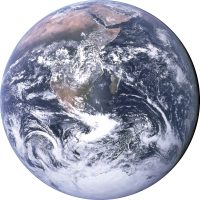
\includegraphics[height=1cm]{bluemarble}}
\chead{\headmark}
\automark{section}
%\ihead{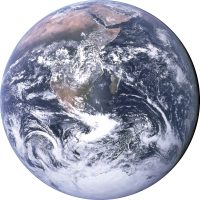
\includegraphics[height=1cm]{bluemarble.jpg}}
\ifoot{\csname @title\endcsname}\cfoot{\pagemark}
\ofoot{\today}

\begin{document}
%%%%% BEGINN TITEL %%%%%
\title{Prüfungsleistungen und Bewertungskriterien}
\subtitle{Entwicklungsmethoden für Nachhaltige Produkte}
\author{Abhishek Gupta \and Ludger Heide}
\maketitle
%%%%% ENDE TITEL %%%%%

\tableofcontents

%%%%% BEGINN INHALT %%%%%

\section{Über dieses Dokument}

\section{Prüfungsleistungen}

\begin{table}
	\centering
	\caption{Zusammensetzung der Gesamtnote}
	\label{tab:zusammensetzung}
	\begin{tabular}{lrr}
		\toprule
		Name & Typ & Gewichtung \\
		\midrule
		Lernjournal & individuell & 50 \% \\		
		Präsentation & Gruppe & 10 \% \\
		Projektbericht & Gruppe & 40 \% \\	
		\bottomrule
	\end{tabular}
\end{table}

Die Veranstaltung ist als Portfolioprüfung\footnote{Rahmenbedingugen: \href{https://www.tu-berlin.de/asv/menue/gremien/kommissionen_des_as/hinweise_zur_allgstupo/hinweise_zu_portfoliopruefungen/}{\underline{hier}}} konzipiert. Tabelle \ref{tab:zusammensetzung} zeigt die Zusammensetzung der Gesamtnote auf die einzelnen Teilleistungen.

\begin{table}
	\centering
	\caption{Notenschlüssel}
	\label{tab:notenschlüssel}
	\begin{tabular}{lr}
		\toprule
		Punktzahl & Note \\
		\midrule
		$\geq$ 85 & 1,0 \\
		$\geq$ 80 & 1,3 \\
		$\geq$ 75 & 1,7 \\
		$\geq$ 70 & 2,0 \\
		$\geq$ 65 & 2,3 \\
		$\geq$ 60 & 2,7 \\
		$\geq$ 55 & 3,0 \\
		$\geq$ 50 & 3,3 \\
		$\geq$ 45 & 3,7 \\
		$\geq$ 40 & 4,0 \\
		$<$ 40  & 5,0 \\
		\bottomrule
	\end{tabular}
\end{table}

Zur Zuordnung der Portfoliopunkte zu den Noten kommt der "`Notenschlüssel 3"' der Fakultät IV zur Anwendung, wie in Tabelle \ref{tab:notenschlüssel} gezeigt. Dieser Notenschlüssel ist "`großzügiger"' als die üblicherweise an der Fakultät V verwendeten. Wir wollen eine Lehrveranstaltung, in der "`sehr gut"' nicht "`fehlerfrei"' bedeuten muss und wir nicht eine Korrektur für die Punkte machen und eine, in der wir alle Fehler auszählen, die uns zwar aufgefallen sind aber für die wir keine Punkte abziehen können, weil sonst die Note zu schlecht wird. Studierende sollten also damit rechnen, das die Punktzahlen der Teilleistungen schlechter als gewohnt ausfallen, die Noten jedoch nicht.

\subsection{Lernjournal}

\subsubsection{Beschreibung}

\subsubsection{Bewertungskriterien}

\subsection{Präsentation}

\subsubsection{Beschreibung}

\subsubsection{Bewertungskriterien}

\subsection{Projektbericht}

\subsubsection{Beschreibung}

\subsubsection{Bewertungskriterien}


%%%%% ENDE INHALT %%%%%

%Bibliographie
%\printbibliography

\end{document}
